The discrete system \eqref{eq:DGMPM_discrete_RK2} is now specialized to a one-dimensional problem for which $s_1>0$.
Thus, a domain of length $l$ is divided with $N_p$ material points arbitrarily distributed in $E$ two-node elements of constant length $\Delta x$ (figure~\ref{fig:1Dmesh}).
The grid mesh is such that at least one particle lies in every cell during the computation in order to ensure that there is no hole.
Moreover, periodic boundary conditions are considered to simplify the analysis.
\begin{figure}[h!]
  \centering
  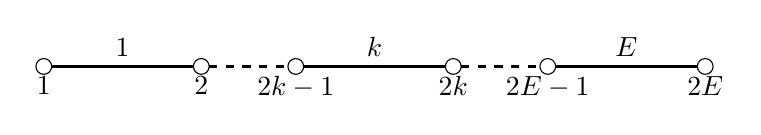
\begin{tikzpicture}
  \draw (2.3,0) circle (0.1) node [below] {$1$};
  \draw (4.3,0) circle (0.1) node [below] {$2$};
  \draw[thick] (2.4,0) -- (4.2,0) node [above,midway] {$1$};
  \draw[thick,dashed] (4.4,0) -- (5.4,0);
  \draw (5.5,0) circle (0.1) node [below] {$2k-1$};
  \draw (7.5,0) circle (0.1) node [below] {$2k$};
  \draw[thick] (5.6,0) -- (7.4,0) node [above,midway] {$k$};
  \draw[thick,dashed] (7.6,0) -- (8.6,0);
  \draw (8.7,0) circle (0.1) node [below] {$2E-1$};
  \draw (10.7,0) circle (0.1) node [below] {$2E$};
  \draw[thick] (8.8,0) -- (10.6,0) node [above,midway] {$E$};
\end{tikzpicture}

  \caption{One-dimensional mesh made of $E$ elements of constant length $\Delta x = \frac{l}{E}$.}\label{fig:1Dmesh}
\end{figure}
In that mesh, the cell containing the particle $I$ is denoted by $c(I)$ so that the nodes interacting with this particle are $2c(I)-1$ and $2c(I)$.
Since only scalar quantities are considered here, subscript can be used to denote nodal or particle values without ambiguity.
Therefore, the linear shape functions defined in element $c(I)$ are:
\begin{equation}
S_{2c(I)-1}(x)= \frac{x_{2c(I)} - x}{\Delta x} \: ; \: S_{2c(I)}(x)= \frac{x -x_{2c(I)-1}}{\Delta x} \quad x \in \[x_{2c(I)-1},x_{2c(I)}\]
\end{equation}
and $S_{iI}$ or $S_{i,I}$ correspond to the shape function of node $i$ evaluated at the position of the $I$th material point.
In order to better distinguish nodal and particle fields, uppercase symbols are used for material point quantities.

\subsection{The scheme equation}
The method followed to write the scheme equation is to trace backward the numerical procedure described in section \ref{sec:dgmpm} to get an expression of the form:
\begin{equation}
  \label{eq:scheme_general}
  \bar{Q}^{k+1}_I=H\(\bar{Q}^{k}_J\) \qquad  J=1,..,N_p
\end{equation}
where $H$ stands for the DGMPM discrete solution operator.

The two stages of the RK2 algorithm can be written as:
\begin{equation}
  \label{eq:RK2_algo}
  \bar{q}^{k+\frac{p+1}{2}}_i  =\bar{q}^{k}_i + \frac{p+1}{2}\frac{\Delta t}{M^L_{i}} s_1 \( \sum_{j=1}^{2E} K_{i,j} \bar{q}^{k+\frac{p}{2}}_j - \hat{F}^{k+\frac{p}{2}}_in_i \), \quad  \text{no sum on $i$}   
\end{equation}
in which $\hat{F}^{k+\frac{p}{2}}_i$ and $n_i=\pm1$ are respectively the intercell flux and the outward unit normal at node $i$, and $p=\{0,1\}$ refers to the two stages of the scheme.
Moreover, the mass density is approximated on the grid as:
\begin{equation}
  \label{eq:grid_density}
  \rho(x) = \frac{M^L_{2c-1}+M^L_{2c}}{\Delta x} = \frac{\sum_{J=1}^{N_p^c} m_J}{\Delta x}, \quad x \in [x_{2c-1},x_{2c}]
\end{equation}
where $N_p^{c}$ is the number of particles in cell $c$.
The mass is uniformly distributed between particles so that the previous definition reduces to $\rho = N_p^{c} m^c/\Delta x$, with $m^c$ the mass carried by particles lying in $c$.

First, quantities at time $t^{k+1}$ at particles are obtained by interpolating nodal solutions of the discrete system \eqref{eq:RK2_algo}: 
\begin{equation}
\bar{Q}^{k+1}_I = S_{2c(I)-1,I}\bar{q}_{2c(I)-1}^{k+1} + S_{2c(I),I}\bar{q}_{2c(I)}^{k+1} \label{eq:updated_MP}
\end{equation}
Second, provided linear shape functions, the lumped mass and the pseudo-stiffness matrices are:
\begin{align}
  & M^L_i = \sum_{J=1}^{N_p} S_{iJ} m_J = m^{c(i)} \sum_{J=1}^{N_p} S_{iJ}\\
  & K_{2c(I)-1,j} = \sum_{J=1}^{N_p} \drond{S_{2c(I)-1,J}}{x} m_J S_{jJ} = -m^{c(i)} \sum_{J=1}^{N_p} \frac{ S_{jJ}}{\Delta x} \\
  & K_{2c(I),j} = \sum_{J=1}^{N_p} \drond{S_{2c(I),J}}{x} m_J S_{jJ} = m^{c(i)}\sum_{J=1}^{N_p} \frac{ S_{jJ}}{\Delta x} 
\end{align}
The discontinuous approximation basis moreover yields a bloc diagonal pseudo-stiffness matrix so that one can write:
\begin{equation}
  \label{eq:block_diag_K}
  K_{ij} \bar{q}_{j}^{k}= K_{i,2c(i)-1} \bar{q}_{2c(i)-1}^{k}+K_{i,2c(i)} \bar{q}_{2c(i)}^{k}
\end{equation}
Third, a right-going wave leads to a stationary solution of Riemann problems equals to the state of the upwind node of an interface, that is:
\begin{align}
  & q_{2c(I)-1}^* = \rho \bar{q}^k_{2c(I)-2}=  N_p^{c(I)}\frac{ m^{c(I)}}{\Delta x}\bar{q}^k_{2c(I)-2} \\
  & q_{2c(I)}^* = \rho \bar{q}^k_{2c(I)} =  N_p^{c(I)}\frac{ m^{c(I)}}{\Delta x} \bar{q}^k_{2c(I)} 
\end{align}
Therefore, gathering all the previous considerations, equation \eqref{eq:RK2_algo} reads for each node of cell $c(I)$:
\begin{equation}
  \label{eq:nodal_RK2}
  \begin{aligned}
    & \bar{q}_{2c(I)-1}^{k+\frac{p+1}{2}}= \bar{q}_{2c(I)-1}^{k} - \frac{p+1}{2}\frac{s_1\Delta t}{\Delta x}\( \frac{f_{c(I)}^{k+\frac{p}{2}} - N_p^{c( I)} \bar{q}^{k+\frac{p}{2}}_{2c(I)-2}}{\sum_{K=1}^{N_p^{c(I)}}S_{2c(I)-1,K}}\)\\
    & \bar{q}_{2c(I)}^{k+\frac{p+1}{2}}= \bar{q}_{2c(I)}^{k} + \frac{p+1}{2}\frac{s_1\Delta t}{\Delta x}\( \frac{f_{c(I)}^{k+\frac{p}{2}} - N_p^{c( I)} \bar{q}^{k+\frac{p}{2}}_{2c(I)}}{\sum_{K=1}^{N_p^{c(I)}}S_{2c(I),K}}\)
    % & \bar{q}_{2c(\alpha)-1}^{k+(k+1)/2}= \bar{q}_{2c(\alpha)-1}^{k+k/2} - \frac{k+1}{2}\frac{a\Delta t}{\Delta x}\( \frac{\sum_{\mu=1}^{N_p^{c(\alpha)}} \[S_{2c(\alpha)-1,\mu}\bar{q}_{2c(\alpha)-1}^{k+k/2}+ S_{2c(\alpha),\mu}\bar{q}_{2c(\alpha)}^{k+k/2}\] - N_p^{c( \alpha)} \bar{q}^{k+k/2}_{2c(\alpha)-2}}{\sum_{\mu=1}^{N_p^{c(\alpha)}}S_{2c(\alpha)-1,\mu}}\)\\
    % & \bar{q}_{2c(\alpha)}^{k+(k+1)/2}= \bar{q}_{2c(\alpha)}^{k+k/2} - \frac{k+1}{2}\frac{a\Delta t}{\Delta x}\( \frac{\sum_{\mu=1}^{N_p^{c(\alpha)}} \[S_{2c(\alpha)-1,\mu}\bar{q}_{2c(\alpha)-1}^{k+k/2}+ S_{2c(\alpha),\mu}\bar{q}_{2c(\alpha)}^{k+k/2}\] - N_p^{c( \alpha)} \bar{q}^{k+k/2}_{2c(\alpha)}}{\sum_{\mu=1}^{N_p^{c(\alpha)}}S_{2c(\alpha),\mu}}\)
  \end{aligned},\quad p=\{0,1\}
\end{equation}
with the volume fluxes contributions $f_{c}^{k}=\sum_{J=1}^{N_p^{c}} \[S_{2c-1,J}\bar{q}_{2c-1}^{k}+ S_{2c,J}\bar{q}_{2c}^{k}\]$.
Note that equation \eqref{eq:nodal_RK2} involves the Courant number $s_1\Delta t/\Delta x$.

The first stage of equation \eqref{eq:nodal_RK2} (\textit{i.e. }$p=0$) yields the intermediate nodal fields in cell $c(I)$:
\begin{equation}
  \label{eq:discrete_RK2_step1}
  \begin{aligned}
    &\bar{q}_{2c(I)-1}^{k+\frac{1}{2}}= \bar{q}_{2c(I)-1}^{k} - \frac{s_1\Delta t}{2\Delta x}\( \frac{f_{c(I)}^{k} - N_p^{c( I)} \bar{q}^k_{2c(I)-2}}{\sum_{K=1}^{N_p^{c(I)}}  S_{2c(I)-1,K}}\)\\
    &\bar{q}_{2c(I)}^{k+\frac{1}{2}}= \bar{q}_{2c(I)}^{k} + \frac{s_1\Delta t}{2\Delta x}\( \frac{f_{c(I)}^{k}- N_p^{c( I)}  \bar{q}^k_{2c(I)}}{\sum_{K=1}^{N_p^{c(I)}}  S_{2c(I),K}} \)
  \end{aligned}
\end{equation}
and the second one (\textit{i.e. }$p=1$) leads to the expression of nodal quantities at the end of the time step:
\begin{equation}
  \label{eq:discrete_RK2_step2}
  \begin{aligned}
    &\bar{q}_{2c(I)-1}^{k+1}= \bar{q}_{2c(I)-1}^{k} - \frac{s_1\Delta t}{\Delta x}\( \frac{\sum_{J=1}^{N_p^{c(I)}}\[S_{2c(I)-1,J}\bar{q}_{2c(I)-1}^{k+\frac{1}{2}}+ S_{2c(I),J}\bar{q}_{2c(I)}^{k+\frac{1}{2}}\] - N_p^{c( I)} \bar{q}^{k+\frac{1}{2}}_{2c(I)-2}}{\sum_{K=1}^{N_p^{c(I)}}  S_{2c(I)-1,K}}\)\\
    &\bar{q}_{2c(I)}^{k+1}= \bar{q}_{2c(I)}^{k} + \frac{s_1\Delta t}{\Delta x}\( \frac{\sum_{J=1}^{N_p^{c(I)}}\[S_{2c(I)-1,J}\bar{q}_{2c(I)-1}^{k+\frac{1}{2}}+ S_{2c(I),J}\bar{q}_{2c(I)}^{k+\frac{1}{2}}\]- N_p^{c( I)}  \bar{q}^{k+\frac{1}{2}}_{2c(I)}}{\sum_{K=1}^{N_p^{c(I)}}  S_{2c(I),K}} \)
  \end{aligned}
\end{equation}
Then, introduction of equations \eqref{eq:discrete_RK2_step2} in the interpolation from nodes to particles \eqref{eq:updated_MP} leads to the solution at material point $I$ and time step $k+1$:
\begin{equation}
  \label{eq:second_stage_MP}
  \begin{split}
    \bar{Q}^{k+1}_I &=  S_{2c(I)-1,I}\bar{q}_{2c(I)-1}^{k}+S_{2c(I),I}\bar{q}_{2c(I)}^{k} +N_p^{c(I)}\frac{s_1\Delta t}{\Delta x}\frac{S_{2c(I)-1,I}}{\sum_{K}  S_{2c(I)-1,K}}\bar{q}_{2c(I)-2}^{k+\frac{1}{2}} \\
    &- \(\frac{s_1\Delta t}{\Delta x}\[S_{2c(I)-1,I} - S_{2c(I),I}\frac{\sum_{J} S_{2c(I)-1,J}}{\sum_{K}  S_{2c(I),K}}\] \)\bar{q}_{2c(I)-1}^{k+\frac{1}{2}} \\
    & + \frac{s_1\Delta t}{\Delta x}\[S_{2c(I),I} - S_{2c(I)-1,I}\frac{\sum_{J} S_{2c(I),J}}{\sum_{K}  S_{2c(I)-1,K}}- N_p^{c(I)}\frac{S_{2c(I),I}}{\sum_{K}  S_{2c(I),K}}\] \bar{q}_{2c(I)}^{k+\frac{1}{2}}
  \end{split}
\end{equation}
Nodal values $\bar{q}_i^{k+\frac{1}{2}}$ are provided by the first stage of RK2 algorithm and can be substituted the above equation: %in equation \eqref{eq:second_stage_MP}:
\begin{equation}
  \begin{split}
    \bar{Q}^{k+1}_I &=  S_{2c(I)-1,I}\bar{q}_{2c(I)-1}^{k} +S_{2c(I),I}\bar{q}_{2c(I)}^{k} +N_p^{c(I)}\frac{s_1\Delta t}{\Delta x}\frac{S_{2c(I)-1,I}}{\sum_{K}  S_{2c(I)-1,K}}\(\bar{q}_{2c(I)-2}^{k} + \frac{s_1\Delta t}{2\Delta x}\( \frac{f_{c(I)-1}^{k}- N_p^{c( I)}  \bar{q}^k_{2c(I)-2}}{\sum_{K}  S_{2c(I)-2,K}} \)\)\\
    -& \frac{s_1\Delta t}{\Delta x}\[S_{2c(I)-1,I} - S_{2c(I),I}\frac{\sum_{J} S_{2c(I)-1,J}}{\sum_{K}  S_{2c(I),K}}\] \(\bar{q}_{2c(I)-1}^{k} - \frac{s_1\Delta t}{2\Delta x}\( \frac{f_{c(I)}^{k} - N_p^{c( I)} \bar{q}^k_{2c(I)-2}}{\sum_{K}  S_{2c(I)-1,K}}\)\) \\
    +& \frac{s_1\Delta t}{\Delta x}\[S_{2c(I),I}\(1- \frac{N_p^{c(I)}}{\sum_{K}  S_{2c(I),K}}\) - S_{2c(I)-1,I}\frac{\sum_{J} S_{2c(I),J}}{\sum_{K}  S_{2c(I)-1,K}}\] \(\bar{q}_{2c(I)}^{k} + \frac{s_1\Delta t}{2\Delta x}\( \frac{f_{c(I)}^{k}- N_p^{c( I)}  \bar{q}^k_{2c(I)}}{\sum_{K}  S_{2c(I),K}} \)\)
    \label{eq:Mp_before_mapping}
  \end{split}
\end{equation}
Note that the solution of the downstream node of the adjacent cell $\bar{q}^{k+\frac{1}{2}}_{2c(I)-2}$ results from the second equation of the set \eqref{eq:discrete_RK2_step1}.
Therefore, by rearranging formula \eqref{eq:Mp_before_mapping}:
%Note that the second equation of the set \eqref{eq:discrete_RK2_step1} is used for $q^{k+\frac{1}{2}}_{2c(J)-2}$ since it is the downwstream node of the adjacent cell $c(J)-1$. At last, by rearranging formula \eqref{eq:Mp_before_mapping} as:
\begin{equation}
  \label{eq:euler_before_mapping}
  \begin{split}
    \bar{Q}^{k+1}_I =  &\(S_{2c(I)-1,I} -\frac{s_1\Delta t}{\Delta x}\[S_{2c(I)-1,I} - S_{2c(I),I}\frac{\sum_{J} S_{2c(I)-1,J}}{\sum_{K}  S_{2c(I),K}}\]\)\bar{q}_{2c(I)-1}^{k} \\
    +&\(S_{2c(I),I} + \frac{s_1\Delta t}{\Delta x}\[S_{2c(I),I}\(1-\frac{N_p^{c(I)}}{\sum_{K}  S_{2c(I),K}}\) - S_{2c(I)-1,I}\frac{\sum_{J} S_{2c(I),J}}{\sum_{K}  S_{2c(I)-1,K}}\]\) \bar{q}_{2c(I)}^{k} \\
    +&\frac{1}{2}\(\frac{s_1\Delta t}{\Delta x}\)^2\(N_p^{c( I)}\[\frac{S_{2c(I)-1,I}}{\sum_K S_{2c(I)-1,K}} - \frac{S_{2c(I),I}}{\sum_{K}  S_{2c(I),K}}\] +S_{2c(I),I} \(\frac{N_p^{c(I)}}{\sum_{K}  S_{2c(I),K}}\)^2\)\bar{q}_{2c(I)}^{k}\\
    +&N_p^{c( I)}\frac{s_1\Delta t}{\Delta x}  \[ \frac{S_{2c(I)-1,I}}{\sum_{K}  S_{2c(I)-1,K}}\(1 -   \frac{s_1\Delta t}{2\Delta x}\(1+\frac{N_p^{c( I)} }{\sum_{K}  S_{2c(I)-2,K}} \)\)+\frac{s_1\Delta t}{2\Delta x} \frac{S_{2c(I),I}}{\sum_{K}  S_{2c(I),K}}\]\bar{q}^k_{2c(I)-2}\\
    -&\frac{1}{2}\(\frac{s_1\Delta t}{\Delta x}\)^2 N_p^{c(I)}\frac{S_{2c(I),I}}{\(\sum_{K}  S_{2c(I),K}\)^2} f_{c(I)}^{k} +\frac{1}{2}\(\frac{s_1\Delta t}{\Delta x}\)^2N_p^{c(I)}\frac{S_{2c(I)-1,I}}{\sum_{K}  S_{2c(I)-1,K}}\frac{ f_{c(I)-1}^{k}}{\sum_{K}  S_{2c(I)-2,K}}
  \end{split}
\end{equation}

Next, the nodal solutions at time step $k$ in equation \eqref{eq:euler_before_mapping} result from the projection between particles and the grid \eqref{eq:DGMPM_points2nodes}:
%In equation \eqref{eq:euler_before_mapping} the solutions at nodes result from the convection step \eqref{eq:DGMPM_points2nodes}:
\begin{equation}
\bar{q}^{k}_{i} = \frac{\sum_L S_{iL}m_L \bar{Q}^k_{L}}{\sum_K S_{iK}m_K} = \frac{\sum_L S_{iL} \bar{Q}^k_{L}}{\sum_K S_{iK}} \label{eq:stab_mapping}
\end{equation}
In particular, volume fluxes contributions can be written:
\begin{equation}
  \label{eq:volume_fluxes_mapped}
  \begin{aligned}
    f_{c}^{k}&=\sum_{J=1}^{N_p^{c}}\[S_{2c-1,J}\frac{\sum_L S_{2c-1,L}\bar{Q}^k_{L}}{\sum_K S_{2c-1,K}}+ S_{2c,J}\frac{\sum_L S_{2c,L} \bar{Q}^k_{L}}{\sum_K S_{2c,K}} \]\\
    f_{c}^{k}&=\sum^{N_p}_{L=1}\(S_{2c-1,L} +S_{2c,L} \)\bar{Q}^k_{L}  \\ 
    f_{c}^{k}&=\sum^{}_{L \in c}\bar{Q}^k_{L}   
  \end{aligned}
\end{equation}
where the partition of unity yields the last equality.

The use of mapping equations \eqref{eq:stab_mapping} and \eqref{eq:volume_fluxes_mapped} allows to write after some simplifications:
% \begin{equation}
%   \begin{split}
%     \bar{Q}^{k+1}_I =  &\sum_{L} \bar{Q}_L^k  \left\lbrace \frac{S_{2c(I)-1,L}}{\sum_K S_{2c(I)-1,K}}\(S_{2c(I)-1,I} -\frac{s_1\Delta t}{\Delta x}\[S_{2c(I)-1,I} - S_{2c(I),I}\frac{\sum_{J} S_{2c(I)-1,J}}{\sum_{K}  S_{2c(I),K}}\]\)  \right. \\
%     &+\frac{S_{2c(I),L}}{\sum_K S_{2c(I),K}}\(S_{2c(I),I} + \frac{s_1\Delta t}{\Delta x}\[S_{2c(I),I}\(1-\frac{N_p^{c(I)}}{\sum_{K}  S_{2c(I),K}}\) - S_{2c(I)-1,I}\frac{\sum_{J} S_{2c(I),J}}{\sum_{K}  S_{2c(I)-1,K}}\]\)  \\
%     &+\frac{S_{2c(I),L}}{\sum_K S_{2c(I),K}}\frac{1}{2}\(\frac{s_1\Delta t}{\Delta x}\)^2\(N_p^{c(I)}\[\frac{S_{2c(I)-1,I}}{\sum_K S_{2c(I)-1,K}} - \frac{S_{2c(I),I}}{\sum_{K}  S_{2c(I),K}}\] +S_{2c(I),I} \(\frac{N_p^{c(I)}}{\sum_{K}  S_{2c(I),K}}\)^2\)  \\
%     &+\frac{N_p^{c(I)} S_{2c(I)-2,L}}{\sum_K S_{2c(I)-2,K}}\frac{s_1\Delta t}{\Delta x} \[ \frac{S_{2c(I)-1,I}}{\sum_{K}  S_{2c(I)-1,K}}\(1 -   \frac{s_1\Delta t}{2\Delta x}\(1+\frac{N_p^{c(I)} }{\sum_{K}  S_{2c(I)-2,K}} \)\)+\frac{s_1\Delta t}{2\Delta x} \frac{S_{2c(I),I}}{\sum_{K}  S_{2c(I),K}}\]\\
%     &+\frac{1}{2}\(\frac{s_1\Delta t}{\Delta x}\)^2 N_p^{c(I)}\left.\( \frac{S_{2c(I)-2,L} +S_{2c(I)-3,L} }{\sum_{K}  S_{2c(I)-1,K}\sum_{K}  S_{2c(I)-2,K}} S_{2c(I)-1,I}-\frac{S_{2c(I)-1,L} +S_{2c(I),L} }{\(\sum_{K}  S_{2c(I),K}\)^2} S_{2c(I),I}\)  \right\rbrace
%   \end{split}
% \end{equation}
% Once the previous formula is simplified, the one-dimensional scheme equation of the DGMPM with the RK2 time discretization can be written:
\begin{equation}
  \label{eq:RK2_scheme}
  \begin{split}
    \bar{Q}^{k+1}_I =  &\sum_{L} \bar{Q}_L^k  \left\lbrace \sum_i S_{iL}\frac{S_{iI}}{\sum_K S_{iK}}
      +\frac{s_1\Delta t}{\Delta X}\[\frac{S_{2c(L),I}}{\sum_{K}  S_{2c(L),K}} - \frac{S_{2c(L)-1,I}}{\sum_{K}  S_{2c(L)-1,K}}\] \right.\\
    &+\frac{s_1\Delta t}{\Delta X}N_p^{c( I)}\[\frac{S_{2c(I)-1,I}}{\sum_{K}  S_{2c(I)-1,K}}\frac{S_{2c(I)-2,L}}{\sum_K S_{2c(I)-2,K}}-\frac{S_{2c(I),I}S_{2c(I),L}}{\(\sum_K S_{2c(I),K}\)^2}\] \\
    &+\frac{1}{2}\(\frac{s_1\Delta t}{\Delta X}\)^2N_p^{c( I)} \(\frac{S_{2c(I),L}}{\sum_K S_{2c(I),K}}-\frac{S_{2c(I)-2,L}}{\sum_K S_{2c(I)-2,K}}\)\[\frac{S_{2c(I)-1,I}}{\sum_K S_{2c(I)-1,K}} - \frac{S_{2c(I),I}}{\sum_{K}  S_{2c(I),K}}\]\\
    &+\frac{1}{2}\(\frac{s_1\Delta t}{\Delta X}\)^2N_p^{c( I)}\frac{S_{2c(L),I}}{\(\sum_{K}  S_{2c(I),K}\)^2} \[N_p^{c( I)}\frac{S_{2c(I),L} }{\sum_K S_{2c(I),K}}-1\]\\
    &+ \frac{1}{2}\(\frac{s_1\Delta t}{\Delta X}\)^2\frac{S_{2c(L)+1,I}N_p^{c(I)}}{\sum_{K}  S_{2c(I)-1,K}\sum_{K}  S_{2c(I)-2,K}} \left.\[ 1 - N_p^{c( I)}\frac{S_{2c(I)-2,L} }{\sum_{K}  S_{2c(I)-2,K}}\] \right\rbrace
    \end{split}
\end{equation}
The three first terms of the latter scheme equation correspond to that obtained for the Euler algorithm \cite{DGMPM}, whereas the second-order terms are provided by the two-stage time integration.
% The brackets in those higher-order corrections vanish when only one point is in each cell of the grid, so that the scheme is equivalent to the well-known first-order upwind method. %% Add comments
% This property of the DGMPM has already been observed for the Euler time discretization \cite{DGMPM}.
Alternatively and given the compact support of shape functions, equation \eqref{eq:RK2_scheme} can be split into two sums, one over the material points contained in the cell $c(I)$, and one over these of cell $c(I)-1$:
\begin{equation}
  \label{eq:RK2_scheme_split}
  \begin{split}
    \bar{Q}^{k+1}_I &=  \sum_{L\in c(I)} \bar{Q}_L^k  \left\lbrace \sum_i S_{iL}\frac{S_{iI}}{\sum_K S_{iK}}
      +\frac{s_1\Delta t}{\Delta X}\[\frac{S_{2c(L),I}}{\sum_{K}  S_{2c(L),K}} - \frac{S_{2c(L)-1,I}}{\sum_{K}  S_{2c(L)-1,K}} - N_p^{c( I)}\frac{S_{2c(I),I}S_{2c(I),L}}{\(\sum_K S_{2c(I),K}\)^2}\] \right.\\
    &\left.+\frac{1}{2}\(\frac{s_1\Delta t}{\Delta X}\)^2N_p^{c( I)} \frac{S_{2c(I),L}}{\sum_K S_{2c(I),K}}\[\frac{S_{2c(I)-1,I}}{\sum_K S_{2c(I)-1,K}} - \frac{S_{2c(I),I}}{\sum_{K}  S_{2c(I),K}}+ N_p^{c( I)}\frac{S_{2c(I),L} }{\(\sum_K S_{2c(I),K}\)^2}-\frac{1}{\sum_K S_{2c(I),K}}\]\right\rbrace\\
    %%%% OTHER SUM
    &+ \sum_{L\in c(I)-1} \bar{Q}_L^k  N_p^{c( I)}\left\lbrace  
      \frac{s_1\Delta t}{\Delta X}\frac{S_{2c(I)-1,I}}{\sum_{K}  S_{2c(I)-1,K}}\frac{S_{2c(L),L}}{\sum_K S_{2c(L),K}} \right. \\
    % &-\frac{1}{2}\(\frac{s_1\Delta t}{\Delta X}\)^2 \frac{S_{2c(L),L}}{\sum_K S_{2c(L),K}}\[\frac{S_{2c(I)-1,I}}{\sum_K S_{2c(I)-1,K}} - \frac{S_{2c(I),I}}{\sum_{K}  S_{2c(I),K}}\]\\
    % &+ \frac{1}{2}\(\frac{s_1\Delta t}{\Delta X}\)^2\frac{S_{2c(L)+1,I}}{\sum_{K}  S_{2c(I)-1,K}} \left.\[\frac{ 1}{\sum_{K}  S_{2c(L),K}} - \frac{S_{2c(L),L} N_p^{c( I)}}{\(\sum_{K}  S_{2c(L),K}\)^2}\] \right\rbrace
    %% TEST FOR LAST TWO LINES
    & \left.+ \frac{1}{2}\(\frac{s_1\Delta t}{\Delta X}\)^2\(\frac{S_{2c(L)+1,I}}{\sum_{K}  S_{2c(I)-1,K}} \[\frac{ 1}{\sum_{K}  S_{2c(L),K}} - \frac{S_{2c(L),L} N_p^{c( I)}}{\(\sum_{K}  S_{2c(L),K}\)^2}\]-\frac{S_{2c(L),L}}{\sum_K S_{2c(L),K}}\[\frac{S_{2c(I)-1,I}}{\sum_K S_{2c(I)-1,K}} - \frac{S_{2c(I),I}}{\sum_{K}  S_{2c(I),K}}\]\)\right\rbrace
    \end{split}
\end{equation}
When only one point lies in each cell of the grid, the sum of shape functions over particles reduces to one single term (\textit{e.g. }$\sum_{K}  S_{2c(J)-1,K} = S_{2c(J)-1,J}$).
Thus, one can show that the terms under brackets in the above equation all vanish so that the scheme reduces to:
\begin{equation}
  \label{eq:RK2_1ppc}
  \bar{Q}^{k+1}_I=  (1-\frac{s_1\Delta t}{\Delta X})\bar{Q}_I^k+\frac{s_1\Delta t}{\Delta X}\bar{Q}_{I-1}^k
\end{equation}
%which corresponds to the well-known first-order upwind method.
It then appears that, as for the DGMPM combined with the Forward Euler time integration \cite{DGMPM}, the use of one particle per cell and RK2 time discretization within the DGMPM leads, for one-dimensional problems, to the well-known first-order upwind method.
%Thus, assuming that the approximation leads to an order of accuracy greater than one, a first-order of accuracy can be achieved by adapting only the space discretization and the polynomial order.
%This is an interesting feature of the scheme in order to capture discontinuities.
% This result highlights an interesting feature of the DGMPM which consists in allowing to modify the order of the method by only changing the space discretization.
%Indeed, assuming that the approximation leads to an order of accuracy greater than one, the use of only one particle and linear shape functions in a cell enables to locally achieve first order accuracy even for a second-order time integration.
%Hence, if the cell is known to be crossed by a discontinuity, the required first-order can be reached so as to capture the jump.

\subsection{The von Neumann linear stability analysis}

The scheme equation \eqref{eq:RK2_scheme} is written for simplicity:
\begin{equation}
\bar{Q}^{k+1}_I = \sum_{L=1}^{N_p}  H_{IL} \bar{Q}^k_{L}\label{eq:scheme_Dpi}
\end{equation}
Moreover, the computational domain is repeated periodically by mapping it to the domain $[-l,0]$ so that the solution at material point $I$ and time step $k$ is expanded into a discrete Fourier basis of $2E+1$ harmonics over the domain $x \in \[-l,l\]$:
\begin{equation}
\bar{Q}^{k}_I = \sum_{j=-E}^{E}A_j^k e^{i I \lambda_j \Delta x}
\end{equation}
with $A^k_j$, the magnitude of the $j$th harmonic at time step $k$, $i = \sqrt{-1}$, and $\lambda_j$ the wave number.
Introduction of this expansion in equation \eqref{eq:scheme_Dpi} yields:
\begin{equation}
A_j^{k+1} e^{iI \lambda_j \Delta x} = \sum_{L=1}^{N_p} A_j^k H_{IL}e^{i L \lambda_j \Delta x}\quad \forall j=-E,...,E
\end{equation}
The amplification factor between two time steps at a given point is defined as:
\begin{equation}
\frac{A_j^{k+1}}{A_j^k} = \sum_{L=1}^{N_p} e^{i (L -I)\lambda_j \Delta x} H_{IL} \quad \forall j=-E,...,E \label{eq:fourier_expansion}
\end{equation}
A necessary condition to ensure the stability of a numerical scheme is that the amplification factor must be lower than or equal to one in modulus: $\abs{A^{k+1}/A^k} \leq 1$.
This upper bound allows to prevent an increasing error during the computation. For expression \eqref{eq:fourier_expansion}, this leads to:
\begin{equation}
 \abs{\sum_{L=1}^{N_p} e^{i (L -I)\lambda_j \Delta x} H_{IL}} \leq \sum_{L=1}^{N_p} \abs{e^{i (L -I)\lambda_j \Delta x} H_{IL}} = \sum_{L=1}^{N_p} \abs{H_{IL}} \quad \forall j=-E,...,E
\end{equation}
where the triangle inequality, and the unit modulus of the complex number $e^{i (L -I)\lambda_j \Delta x}$ have been used.
Hence, the DGMPM scheme is stable for a given discretization if the Courant number is set so that the following condition is satisfied for all material points:
\begin{equation}
  \label{eq:stability} \sum_{L=1}^{N_p} \abs{H_{IL}} \leq 1 \quad \forall \: I = 1,...,N_p
\end{equation}
The stability of the scheme is thus ensured by using the lowest CFL number satisfying \eqref{eq:stability}.
Note however that the use of the triangle inequality leads to a more severe constraint than that really admissible.
As a consequence, the Courant number can be set in practice to higher values than that resulting from the solution of \eqref{eq:stability}. 

\subsection{Evaluation of the CFL number for particular space discretizations}
%According to the scheme equation \eqref{eq:RK2_scheme},

The stability condition \eqref{eq:stability} can be very hard to solve analytically for general discretizations.
Nevertheless, the Courant number can be set to unity for one particle lying in every cells, regardless of their positions, since in that case the DGMPM scheme identifies to the first-order upwind method.
On the other hand, though the infinity of possible material points distributions prevents the explicit derivation of a general stability condition, the optimal CFL number satisfying the equality in \eqref{eq:stability} can be found numerically.
Some configurations are studied in table \ref{tab:CFL_comparison} where the critical Courant number resulting from the two time discretizations studied above are compared.
Those results have been obtained by using the same particles distribution in every elements of a one-dimensional regular mesh. 
%
The following configurations are considered:
\begin{itemize}
\item[(i)] particles are positioned symmetrically with respect to cells centers and regularly spaced in the mesh. This space discretization is referred to as the natural configuration in the following.
\item[(ii)] particles in the natural configuration are all shifted of $u=\Delta x/10$.
\item[(iii)] the same than (ii) with $u$ so that one material point overlaps every left nodes of cells.
\item[(iv)] the same than (iii) for right nodes.
\item[(v)] particles are placed symmetrically with respect to cells centers but not regularly spaced in the mesh. Material points in the left half of cells are shifted of $u_1=-\Delta x/10$ while those in the right half are shifted of $u_2=\Delta x/10$.
\item[(vi)] the same than (v) with the first and last particles overlapping left and right nodes of cells respectively.
\end{itemize}


\begin{table}[h!]
  \centering
  \begin{tabular}[ht]{cccccN}
  \hline
  \multicolumn{2}{c}{Number of particles} & Position of $I$th particle in cell $c$ & Euler CFL & RK2 CFL &\\[6pt]
  \hline
  \hline
  (--) &1 &$X^1 \in \[X^{2c-1},X^{2c}\]$  &  1 & 1&\\[8pt]
  \hline
  (i)& 2 & $ X^I= X^{2c-1}+(2I-1)\frac{\Delta X}{4}$ &  0.43 & 1&\\[8pt]
  (ii)& 2 & $X^I= X^{2c-1}+(2I-1)\frac{\Delta X}{4} +\frac{\Delta X}{10} $ &  0.40 & 0.50 &\\[8pt]
  (iii)& 2 & $X^I= X^{2c-1}+(2I-1)\frac{\Delta X}{4} +(I-2)\frac{\Delta X}{10} $ &  0.27 & 1 &\\[8pt]
  (iii)'& 2 & $X^I= X^{2c-1}+(2I-1)\frac{\Delta X}{4} +(I-2)\frac{\Delta X}{4} $ &  0 & 1 &\\[8pt]
  \hline
  (i)& 3 & $ X^I= X^{2c-1}+2I\frac{\Delta X}{8}$ &  0.43 & 1&\\[8pt]
  (ii)& 3 & $X^I= X^{2c-1}+2I\frac{\Delta X}{8} +\frac{\Delta X}{10} $ &  0.40 & 0.50 &\\[8pt]
  (iii)& 3 & $X^I= X^{2c-1}+2I\frac{\Delta X}{8} +(I-2)\frac{\Delta X}{10} $ &  0.27 & 1 &\\[8pt]
  (iii)'& 3 & $X^I= X^{2c-1}+2I\frac{\Delta X}{8} +(I-2)\frac{\Delta X}{4} $ &  0 & 1 &\\[8pt]
  \hline
  (i)& 4 & $ X^I= X^{2c-1}+I\frac{\Delta X}{5}$ &  0.35 & 1&\\[8pt]
  (ii)& 4 & $X^I= X^{2c-1}+I\frac{\Delta X}{5} +\frac{\Delta X}{10} $ &  0.31 & 0.40 &\\[8pt]
  (iii)& 4 & $X^I= X^{2c-1}+I\frac{\Delta X}{5} +\frac{2I-5}{\abs{2I-5}}\frac{\Delta X}{10} $ &  0.18 & 1 &\\[8pt]
  (iii)'& 4 & $X^I= X^{2c-1}+I\frac{\Delta X}{5} +\frac{2I-5}{\abs{2I-5}}\frac{\Delta X}{5} $ &  0 & 1 &\\[8pt]
  \hline
\end{tabular}

%%% Local Variables: 
%%% mode: latex
%%% TeX-master: "../../mainManuscript"
%%% End:
  \caption{DGMPM critical Courant number values for Euler or RK2 time integration for several one-dimensional discretizations. Black circles denote material points while white ones represent grid nodes.}
  \label{tab:CFL_comparison}
\end{table}
First, table \ref{tab:CFL_comparison} shows that the natural configuration leads to the optimal stability bound for the RK2 integrator while the CFL number allowed by using Euler time discretization decreases with increasing number of particles per cell.
Second, moving every points rightward in the mesh (\textit{i.e. cases (ii) and (iv)}) causes a drop in the critical Courant number for both RK2 and Euler algorithms. In particular, stability conditions for more than two particles per cell provided by the RK2 are, in those cases, more restrictive than that of the Euler.
Third, the leftward shifting (\textit{i.e. case (iii)}) leads on the other hand to an improvement of the stability condition for Euler time integration compared to that enabled in the natural configuration.
This property illustrates the upwind nature of the scheme since $s_1>0$.
The CFL number provided by RK2 integration also decreases due to the shifting while remaining higher than Euler one.
At last, particles distributions conserving the symmetry with respect to cells centers (\textit{i.e. cases (v) and (vi)}), yield the optimal stability condition for the RK2 integrator while the Euler CFL depends on the spacing between material points.
More specifically, Euler algorithm leads to a vanishing CFL for the case (vi), thus preventing any simulation.

% Comparison with DGFEM
%\note{2) According to the reviewer "the critical Courant number being similar to the Eulerian DG schemes despite the Lagrangian aspect", make sure that it is true...}
\review{
  Notice that although the stability depends on the position of particles, the optimal Courant number can be reached even with the Euler discretization, whereas the classical DGFEM scheme presented in  \cite{Chavent_Salzano} is restricted to condition $\Delta t / \Delta x = \mathcal{O}(\sqrt{\Delta x})$.
  This limitation has been addressed by introducing slope limiters in order to remove non-physical oscillations in the vicinity of sharp solutions while providing high-order accuracy in smooth regions \cite{Chavent_Cockburn}.
  However, the stability of the method is still bounded by $CFL\leq 1/2$ and the scheme was first-order accurate.
  The use of a second-order Runge-Kutta \cite{DGFEM_CFL} allows to achieve second-order accuracy of the scheme, but the stability condition then reduces to $CFL\leq1/3$.
  It is noteworthy that space-time DGFEM formulations \cite{ST_DGFEM1,ST_DGFEM2} provided more recently the ability to relax constraints of pure space DGFEM and obtained a critical CFL set at 1.
  %
  % Given the applications aimed by the method, which involve discontinuities in finite-deforming solids, the stability properties of DGMPM and DGFEM schemes must be supplemented by the ability of the methods to handle large deformations for a complete comparison.
  % In that context, the DGMPM 
}
%%% Local Variables:
%%% mode: latex
%%% TeX-master: "manuscript"
%%% End:
